%template1.tex
%The following LaTeX source file represents the simplest kind of slide presentation; no overlays, no included graphics. Substitute your favorite style for ``pascal''. To create the PDF file template1.pdf, (1) be sure to use the prosper class, then (2) execute the command latex template1.tex, and (3) the command dvipdf template1.dvi.

%%%%%%%%%%%%%%%%%%%%%%%%%%%%%%% template1.tex %%%%%%%%%%%%%%%%%%%%%%%%%%%%%%%%%%%
\documentclass[a4paper,blends,pdf,colorBG,slideColor]{prosper}
% definitions for slides for CSC544
% Lutz Hamel, (c) 2007

\hypersetup{pdfpagemode=FullScreen}

\usepackage{times}
\usepackage{latexsym}
\usepackage{alltt}
\usepackage{booktabs}
\usepackage{amsmath}
\usepackage{amsopn}
\usepackage{amsfonts}
\usepackage{amssymb}
%\usepackage[usenames]{color}

\def\sign{\qopname\relax{no}{sign}}
\def\argmax{\qopname\relax{no}{argmax}}
\def\argmin{\qopname\relax{no}{argmin}}

\newcommand{\grad}{\ensuremath{\nabla}} 
\newcommand{\loss}{\ensuremath{{\cal L}}}
\newcommand{\err}{\mbox{err}}
\newcommand{\mse}{\mbox{mse}}
\newcommand{\acc}{\mbox{acc}}
\newcommand{\Integer}{\ensuremath{\mathbb{N}}}
\newcommand{\size}[1]{{|{#1}|}}
\newcommand{\Rnspace}[1]{\ensuremath{\mathbb{R}^{#1}}}
\newcommand{\Real}{\ensuremath{\mathbb{R}}}
\newcommand{\mytt}[1]{{\small\tt{#1}}}
\newcommand{\textemph}[1]{{\em #1}}
\newcommand{\suchthat}{\mid}
\newcommand{\orbar}{\;|\;}
\newcommand{\bs}[1]{\begin{slide}{#1}\ptsize{8}}
\newcommand{\es}{\end{slide}}
\newcommand{\co}{\,\colon\;}
\newcommand{\pair}[2]{\ensuremath{( {#1}, {#2} )}}
\newcommand{\model}[1]{\hat{#1}}
\newcommand{\ul}[1]{{\bf\em #1}}
\newcommand{\ol}{\overline}
\newcommand{\definition}[1]{{\bf Definition: }{\em #1}}
\newcommand{\example}[1]{{\bf Example: }{#1}}
\newcommand{\abs}[1]{|{#1}|}
\newcommand{\mytab}{\makebox[.1in]{}}

\newcommand{\fdef}[1]{
\begin{center}
\fbox{
\begin{minipage}{3.5in}
{\bf Definition:}
{#1}
\end{minipage}
}
\end{center}
}

\newcommand{\fframe}[1]{
\begin{center}
\fbox{
\begin{minipage}{3.5in}
{#1}
\end{minipage}
}
\end{center}
}

\newcommand{\nframe}[1]{
\begin{center}
\begin{minipage}{3.5in}
{#1}
\end{minipage}
\end{center}
}

\newenvironment{Rcode}
	{
		\scriptsize
		\begin{quote}
		\begin{alltt}
	}
	{
		\end{alltt}
		\end{quote}
	}




\begin{document}
\bs{Artificial Neural Networks}
Consider the perceptron
\begin{center}
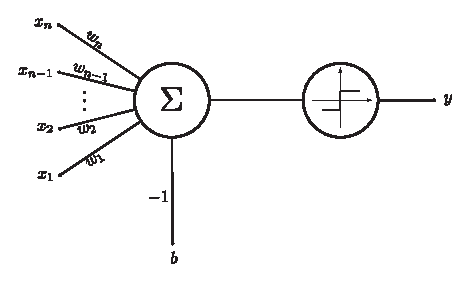
\includegraphics[height=30mm]{figures/fig05-01.eps}
\end{center}
with
\[
\model{f}(\ol{x})= y = \sign\left(\left[\sum_{k=1}^n w_k x_k\right] + (-1) b\right) = \sign\left(\ol{w}\bullet\ol{x} - b\right).
\]
where $\ol{w} = (w_1, w_2, \ldots, w_n)$ and $\ol{x} = (x_1, x_2,\ldots,x_n)$.
The free parameters of the perceptron are $\ol{w}$ and $b$ and they need to be
estimated using some training set $D$.

\es


\bs{Perceptron Learning}
\begin{center}
\fbox{
\begin{minipage}{3in}
{\small
{\bf let} $D = \{(\ol{x}_1,y_1), (\ol{x}_2,y_2),\dots,(\ol{x}_l,y_l)\} \subset \Rnspace{n} \times \{+1, -1\}$\\{\bf let} $0 < \eta <1$\\
$\ol{w} \leftarrow \ol{0}$\\
$b \leftarrow 0$\\
$r \leftarrow \max \{ \abs{\ol{x}} \mid (\ol{x},y)\in D\}$\\
{\bf repeat}\\
\mytab {\bf for} $i = 1$ {\bf to} $l$\\
\mytab\mytab {\bf  if} $\model{f}(\ol{x}_i) \neq y_i$ {\bf then}\\
\mytab\mytab\mytab $\ol{w} \leftarrow \ol{w} +\Delta \ol{w}$\\
\mytab\mytab\mytab $b \leftarrow b - \Delta b$\\
\mytab\mytab {\bf end if}\\
\mytab {\bf end for}\\
{\bf until} $\model{f}(\ol{x}_j) = y_j$ {\rm with} $j = 1,\ldots,l$\\
{\bf return} $(\ol{w}, b)$
}
\end{minipage}
}
\end{center}
where $\Delta \ol{w} =  \eta y_i \ol{x}_i$ and $\Delta b = \eta y_i r^2$.
\es

\bs{Perceptron Learning}

{\bf Problem:} Learning only works for linearly separable data; otherwise the algorithm will not converge.

\vspace{.2in}

Now assume that for the transfer function we use some function $t(\ol{x})$ instead of $\sign(\ol{x})$.

\vspace{.2in}

Also assume that we use the squared error at point $\ol{x}_i$,
\[
se_i =  (y_i - \model{f}(\ol{x}_i))^2
\]
instead of the standard $0-1$ loss function usually associated with classification.  It still gives us the correct classification in the
sense of a loss function:

\begin{quote}
Correct classifications: $(1-1)^2 = 0$ and $((-1) - (-1))^2 = 0$

Incorrect classifications: $(1 - (-1))^2 = 4$ and $((-1) - 1)^2 = 4$
\end{quote}
\es

\bs{Perceptron Learning}
With this we can describe the error of a perceptron at a given point $\ol{x}_i$ with a set of weights $\ol{w}$ as follows,
\[
E_i(\ol{w}) = \frac{1}{2} (y_i - \model{f}(\ol{x}_i))^2 =  \frac{1}{2} (y_i - t(\ol{w}\bullet\ol{x}_i - b))^2
\]
Recall that we swapped out the $sign$ function and replaced with the transfer function $t$.
\es

\bs{Perceptron Learning}
Now that we have a convenient error description we can look at changes of the error in terms of changes of the weights - {\em gradient}.
\[
\grad E_i = (\frac{\partial E_i}{\partial w_1},\cdots,\frac{\partial E_i}{\partial w_n})
\]

\vspace{.2in}

\begin{center}
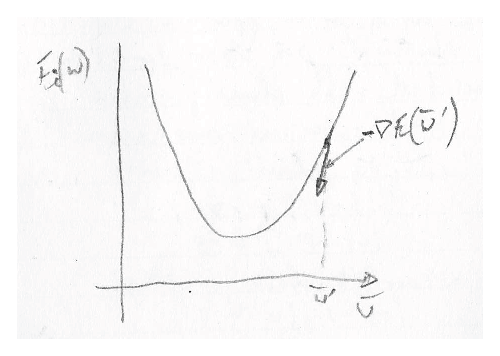
\includegraphics[height=30mm]{images/error-gradient.eps}
\end{center}

This allows us to rewrite our weight update rule $ \ol{w} \leftarrow \ol{w} + \Delta \ol{w}$ with
\[
\Delta \ol{w} = \eta \grad E_i(\ol{w})
\]
\es

\bs{Perceptron Learning}
{\bf Observation:} We no longer try to learn a decision surface that separate the two classes perfectly, instead we are trying to learn a decision
surface that {\em minimizes} the classification error.
\es

\bs{Perceptron Learning}
In order to compute the gradient we need to take the partial derivatives of the error:  The components of $\grad E_i$ are then,
\begin{eqnarray*}
\frac{\partial E_i}{\partial w_j} &=& \frac{\partial}{\partial w_j} \frac{1}{2} (y_i - t(\ol{w}\bullet\ol{x}_i - b))^2\\
	&=& \frac{1}{2} \frac{\partial}{\partial w_j} (y_i - t(\ol{w}\bullet\ol{x}_i - b))^2\\
	&=& - (y_i - t(\ol{w}\bullet\ol{x}_i - b))\frac{\partial t}{\partial w_j} (\ol{w}\bullet\ol{x}_i - b)\\
\end{eqnarray*}
{\bf Observation:} We can only train using the error gradient if the transfer function is differentiable!

\vspace{.2in}

{\bf Note:} The $\sign$ function is {\em not} differentiable because it contains a discontinuity at 0.
\es

\bs{Perceptron Learning}

A convenient transfer function that looks like the $\sign$ function is the $sigmoid$ function,
\[
\sigma(\ol{x}) = \frac{1}{1+e^{-\ol{x}}}
\] 
\begin{center}
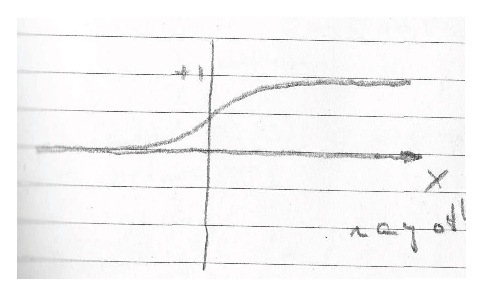
\includegraphics[height=20mm]{images/sigmoid.eps}
\end{center}

Looks like the $\sign$ function but no discontinuities.

\vspace{.2in}

It has a nice derivative,
\[
\frac{d\sigma}{d\ol{x}}(\ol{x}) =  \sigma(\ol{x})(1-\sigma(\ol{x}))
\]
\es

\bs{Perceptron Learning}

What about $b$?

\vspace{.2in}

Here we apply another trick - we embed our training instances $\ol{x} \in R^n$ in a higher dimensional space, namely $R^{n+1}$,
with the embedding function $h$ as follows,
\[
h(\ol{x}) = h(x_1,x_2,\ldots,x_n) = (1,x_1,x_2,\ldots,x_n)
\]
With this our new perceptron looks like this
\begin{center}
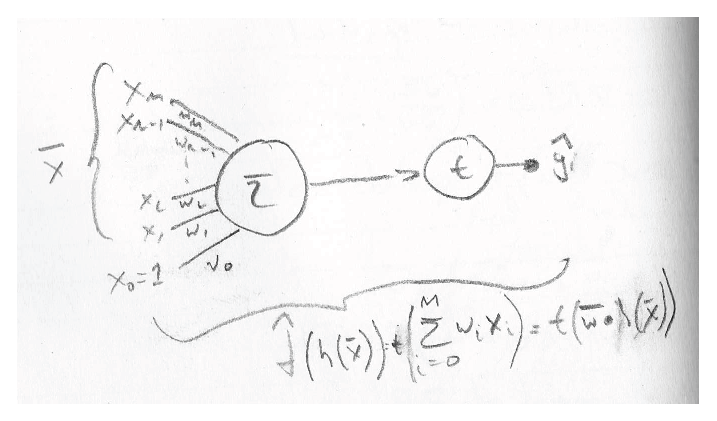
\includegraphics[height=35mm]{images/perceptron.eps}
\end{center}

\es

\bs{Perceptron Learning}

{\bf Observation:} The offset is trained as part of the weight training -- no explicit offset needed.

\vspace{.2in}

{\bf Note:} with $t= sigmoid$ and the embedding function $h$ we talk about single layer ANNs.
\es

\bs{Perceptron Learning}
 Our new training algorithm is as follows,
\begin{center}
\fbox{
\begin{minipage}{3in}
{\small
{\bf let} $D = \{(\ol{x}_1,y_1), (\ol{x}_2,y_2),\dots,(\ol{x}_l,y_l)\} \subset \Rnspace{n} \times \{+1, -1\}$\\{\bf let} $0 < \eta <1$\\
$\ol{w} \leftarrow \ol{0}$\\
{\bf repeat}\\
\mytab {\bf for} $i = 1$ {\bf to} $l$\\
\mytab\mytab\mytab $\ol{w} \leftarrow \ol{w} + \eta \grad E_i(\ol{w})$\\
\mytab {\bf end for}\\
{\bf until} $\grad E(\ol{w}) \approx 0$\\
{\bf return} $\ol{w}$
}
\end{minipage}
}
\end{center}
{\bf Observation:} We don't require the error to be zero, just the gradient.

\vspace{.2in}

\[
\frac{\partial E_i}{\partial w_j} =  - (y_i - t(\ol{w}\bullet h(\ol{x}_i)))\frac{\partial t}{\partial w_j} (\ol{w}\bullet h(\ol{x}_i))
\]
\es


\bs{Multi-Class ANNs}

We can easily extend our single layer ANN to do multi-class classification.  Consider a classification
problem with $k$ classes.  We can construct an ANN for this as follows:

\begin{center}
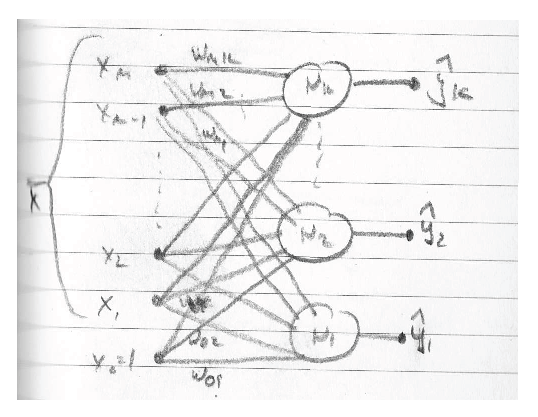
\includegraphics[height=35mm]{images/k-class-perceptron.eps}
\end{center}

We now have $\model{y} = (\model{y}_1,\ldots,\model{y}_k)$ with
\[
\ol{x} \in \mbox{ class } i \mbox{ iff } \model{y} = (0,\ldots,\model{y}_i,\ldots,0) \mbox{ and } y_i = 1.
\]
\es

\bs{Multi-Class ANNs}
Our training data needs to be adjusted to the vector notation of class membership,
\[
D = \{(\ol{x}_1,\ol{y}_1),\ldots,(\ol{x}_l,\ol{y}_l)\} \in R^n\times \{0,1\}^k 
\]

\vspace{.2in}
This means that the multi-class ANN is trained component wise and all our previous result generalize very nicely.
\es

%\bs{Regression with ANNs}
%\begin{center}
%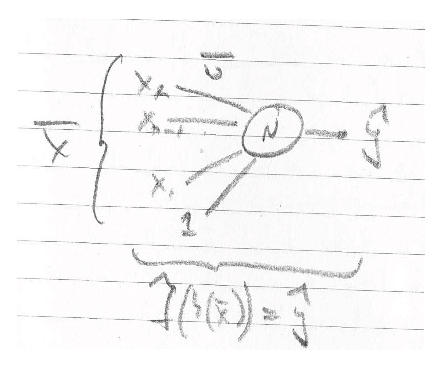
\includegraphics[height=30mm]{images/regression-perceptron.eps}
%\end{center}
%$\model{f}$ is now considered a regression function -- still tries to minimize the squared error but we no longer interpreted the result
%as a loss-function.
%
%\vspace{.2in}
%The difference is in the training set,
%\[
%D = \{(\ol{x}_1,y_1),\ldots,(\ol{x}_l,y_l)\} \in R^n\times R 
%\]
%\es

\bs{Single Layer ANNs}
Problem with single layer ANNs and classification -- only linear decision surface.

\vspace{.2in}

%Problem with single layer ANNs and regression -- only linear regression.
\es
\end{document}
%%%%%%%%%%%%%%%%%%%%%%%%%%% end of template1.tex %%%%%%%%%%%%%%%%%%%%%%%%%%%%%%%%

